\chapter {Descripción y Módulos de Ambienta2MX}
  \section {¿Qué y para qué es Ambienta2MX?}
    \paragraph {\underline{Ambienta2MX} es el nombre de la plataforma que formará parte de una macro solución orientada a la estandarización de metadatos que el INEGI y otras instituciones públicas.}
    \paragraph{Actualmente no existe un estándar de datos geográficos a nivel nacional. Han existido aproximaciones mediante concursos que instituciones públicas como el INEGI ha publicado, o simplemente han existido propuestas que han brindado una solución incompleta a la unión y manejo de información geográfica, geodésica, hidrográfica, climática, topográfica, etc.}
    \paragraph{\underline{Ambienta2MX} toma parte de todo el problema y propone una infraestructura lógica para afrontar la estandarización de variables ambientales y algunos índices de contaminación. Esta información actualmente se encuentra en formatos muy rudimentarios como textos planos sin algún protocolo o formato de interpretación.}
    \paragraph{Sistemas semejantes, por ejemplo, el \textbf{Servicio Meteorológico Nacional} carece de algún recurso del cual se puedan realizar consultas que no sea mediante su portal web, esto trae problemas directos de compatibilidad con otros sitemas. Un caso semejante tenemos con la información que la \textbf{Conagua} maneja en sus centrales meteorológicas a lo largo del país, los datos que brindan se actualizan de forma periodica y el único medio de acceso es a través de una página de internet que devuelve archivos en formato de texto u hojas de cálculo.}
    \paragraph{Los impedimentos antes mencionados conllevan a situaciones tan triviales como la consulta de datos para algúna región o punto específico del territorio nacional, al existir diversas fuentes no es posible tener un compendio del cual tomar la información que más nos convenga. Si a este problema se le añade que los datos carecen de un estandar, llegamos al punto en el que intentar manipular o tratar los datos se vuelve una tarea complicada y en exceso tediosa.}
    \paragraph{Considerando dichos problemas \underline{Ambienta2MX}, propone un estandar de datos climáticos tomando como referencia diversas fuentes y adaptando los tipos de datos a tecnologías y tendencias actuales, brindando así una mayor portabilidad y simplicidad en la consulta de información.}
  \newpage
  \section{Diagrama de Ambienta2MX}
    \paragraph{\underline{Ambienta2MX} constará de varios módulos que trabajarán de forma conjunta para satisfacer la necesidad de tener un estandar y un repositorio de datos climáticos a nivel nacional.}
    \paragraph{Al brindar un sistema modularizado, se genera de forma directa un impacto en el proceso de análisis, desarolló e intengración. Éste tipo de modelo describe de una forma sencilla los componentes necesarios para solventar la demanda a la que se encontrará sometida la plataforma.}
    \paragraph{A continuación se muestra el diagrama a bloques de \underline{Ambienta2MX}, todos los módulos, recursos y bases de datos serán descritos de forma posterior.}
  \newpage
  	\begin{landscape}
	  	\begin{figure}[h!]
	  	\centering
		  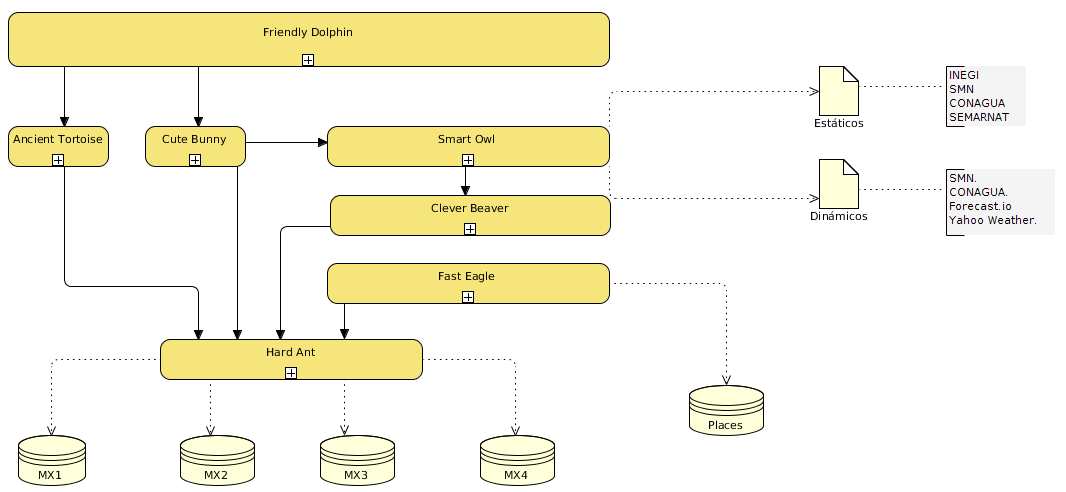
\includegraphics[width=22.5cm,height=12cm]{./images/DiagramaAmbienta2MX.png}
		  \caption{Módulos y estructura de Ambienta2MX}
		\end{figure}
  	\end{landscape}
  \newpage
    \paragraph{Cómo se apreciar en el diagrama, además de los gestores de bases de datos, \underline{Ambienta2MX} se encuentra dividido en siete módulos básicos:}
    \begin{itemize}
		\item Friendy Dolphin.
		\item Ancient Tortoise.
		\item Cute Bunny.
		\item Smart Owl.
		\item Clever Beaver.
		\item Fast Eagle.
		\item Hard Ant.
	\end{itemize}
    \paragraph{En el mismo diagrama se pueden observar las fuentes que proporcionarán la información ya sea a un nivel estático, por ejemplo, carta climática anual de algún municipio del territorio nacional; o bien, recursos que se actualizan de forma periodica como son los datos que provee el Servicio Meteorológico Nacional.}
    \paragraph{Se condieran cinco bases de datos, \emph{MX1, MX2, MX3, MX4, Places}. Todas las bases del tipo MX contarán con la información de variables ambientales así también de los índices de contaminación de las zonas que conforman al territorio nacional.}
    \paragraph{Para el caso de \emph{Places}, la base será usada como un macro índice cartográfico del territorio nacional, es decir, esta base será la referencia a nivel latitud, longitud y altitud para ubicar los datos que requieran ser procesados.}
    \paragraph{Todas las bases se encontrarán funcionando bajo un modelo de base de datos documental teniendo una alimentación bajo demanda, es decir, el contenido gestionado irá aumentando conforme las éstos vayan siendo solicitados.}
\section{Módulos de Ambienta2MX.}
  \subsection{Friendly Dolphin.}
   	\subsubsection{Definición}
   	\paragraph{Éste módulo es el encargado de brindar la información procesada al usuario a través de una página de internet. Es el módo visual que los usuarios finales tendrán para poder interactuar con el ecosistema Ambienta2MX.}
   	\paragraph{Se presenta cómo un módulo web que consumirá la información procesada y almacenada por las cuatro bases (MX1,MX2,MX3,MX4) y la base de soporte (Places).}
   	\paragraph{La principal función es la de consulta y visualización de datos. Es la capa más expuesta y menos técnica de Ambienta2MX ya que es la que tendrá interacción directa con usuarios no técnicos, sin embargo, contará con los procesos necesarios para poder extraer información de las demás plataformas en formatos convencionales cómo JSON, XML o CSV para uso posterior del usuario.}
   	\paragraph{Interactua de forma directa con los bloques \textbf{\emph{Ancient Tortoise}} y \textbf{\emph{Cute Bunny}}, que forman parte de la segunda capa de exposición de datos de Ambienta2MX. Se comunica con los demás módulos mediante servicios de tipo REST que funcionan bajo el patrón de convención sobre configuración\cite{8}, brindando así una gran compatibilidad con éstos además de mejorar el tiempo de desarrollo debido a que no es necesario generar código único y se opta por la reutilización de código y bibliotecas que siguen el mismo método de trabajo.}
	\subsubsection{Diagrama por bloques.}
	\paragraph{Friendly Dolpin contará con varios procesos y módulos a ser desarrollados. Éste módulo se desarrollará usando tecnologías cómo HTML, Javascript y CSS, además de contar con un ciclo continuo de desarrollo usando herramientas de apoyo cómo Yeoman, Gulp para el maquetado y gestión de tareas comunes en projectos de tipo web. A continuación se muestra el diagrama básico de la aplicación.}
  \newpage
  	\begin{landscape}
	  	\begin{figure}[h!]
	  	\centering
		  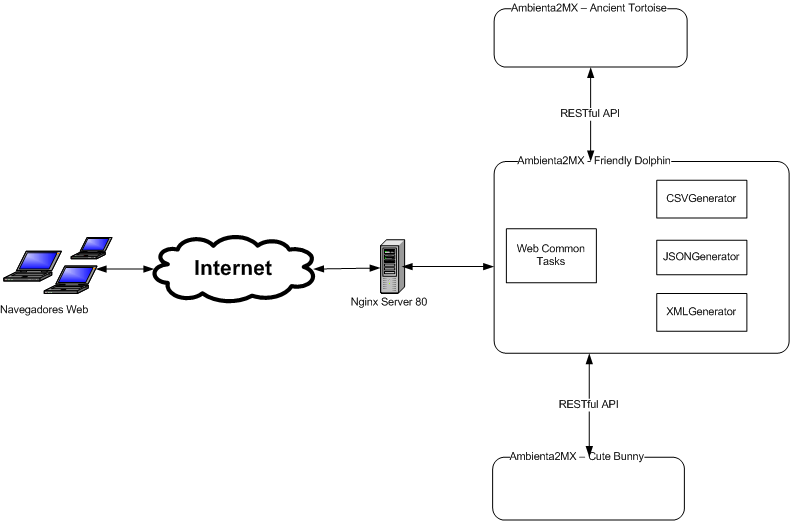
\includegraphics[width=22.5cm,height=12cm]{./images/DiagramaFriendlyDolphin.png}
		  \caption{Diagrama General de Wicked Fox}
		\end{figure}
  	\end{landscape}
  \newpage
  \subsection{Cute Bunny.}
  	\subsubsection{Definición}
  	\subsubsection{Diagrama por bloques.}
  \subsection{Ancient Tortoise.}
  	\subsubsection{Definición}
  	\subsubsection{Diagrama por bloques.}
  \subsection{Smart Owl.}
  	\subsubsection{Definición}
  	\subsubsection{Diagrama por bloques.}
  \subsection{Clever Beaver.}
  	\subsubsection{Definición}
  	\subsubsection{Diagrama por bloques.}
  \subsection{Fast Eagle.}
	  \subsubsection{Definición}
	  	\paragraph{El módulo Fast Eagle formará parte de la arquitectura final de Ambienta2MX. El propósito principal de este módulo es brindar la información cartográfica de México por medio de un servicio expuesto, considerando latitud, longitud o nombre de la localidad deseada.}
  		\paragraph{Fast Eagle se encargará de la lectura, carga, verificación y resolución de los archivos brindados por el (Instituto Nacional de Estadística y Geografía) INEGI en la información pública que tiene de la cartografía del territorio nacional.}
	  	\paragraph{La información que proporciona el INEGI carece de campos esenciales para la estandarización de los datos cartográficos, para dar solución a ese contratiempo se hará uso de servicios externos que ya cuentan con información definida, es decir, que su información ha pasado bajo un cierto proceso de limpieza y regulación, por ejemplo, los servicios de Google Places API y GeoHack.}
	  \subsubsection{Diagrama por bloques.}
	  	\paragraph{Fast Eagle contará con varios procesos a ser desarrollados, la integración de cada proceso y su respectiva integración dará solución a un problema de estandarización, resolución y consulta de datos geográficos vía Latitud, Longitud y Ubicación.}
	  \newpage
	  	\begin{landscape}
		  	\begin{figure}[h!]
		  	\centering
			  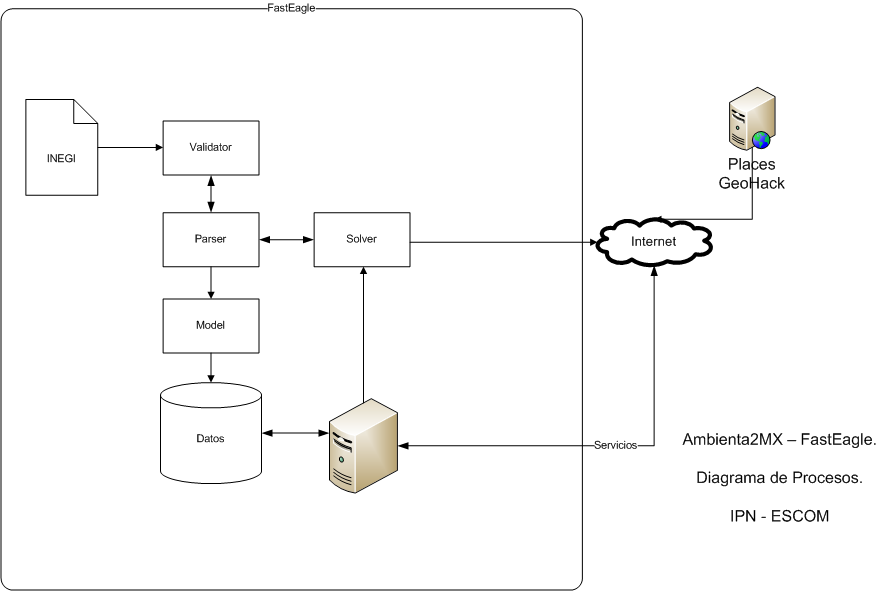
\includegraphics[width=22.5cm,height=12cm]{./images/DiagramaFastEagle.png}
			  \caption{Diagrama General de Fast Eagle}
			\end{figure}
	  	\end{landscape}
	  \newpage
	  \paragraph{En el diagrama se muestran cuatro módulos básicos, estos forman parte del núcleo de Fast Eagle, también podemos observar que se cuenta con la interacción de servicios de terceros como Google Places y GeoHack, también se cuenta con la exposición de los servicios a través de un servidor  web.}
	  \paragraph{El módulo de Validación \textbf{\emph{Validator}}, será el encargado de tomar las fuentes que el INEGI brinda al público en general en forma de archivos CSV, y realizar un proceso de validación a los datos que éstos tienen.}
	  \paragraph{El módulo indicará que datos necesitan una resolución y cuáles pueden ser estandarizados y posteriormente almacenados en la base de datos.}
	  \paragraph{\textbf{\emph{Parser}} tomará los datos que el proceso de validación le arroje para transformar al estado propuesto por el equipo de trabajo (Véase modelo de datos). Considerando un proceso de resolución en caso de que la información proporcionada por el INEGI se encuentre incompleta no sea válida.}
	  \paragraph{Para toda la información que carezca de datos correctos \textbf{\emph{Solver}} buscará una resolución en servicios de terceros, después de la resolución, los datos serán guardados en el gestor de bases de datos bajo el formato propuesto por el equipo de trabajo.}
	  \paragraph{\textbf{\emph{Model}} es la capa de interacción con la base de datos, ésta se encarga de las operaciones mejor conocidas como CRUD (Create, Read, Update and Delete),  persistiendo la información en la base de datos.}
	  \paragraph{Para poder exponer los datos, se hará uso de un servidor web mínimo orientado a micro servicios,  éste será un servicio público que formará parte de la infraestructura final de Ambienta2MX.}
	  \paragraph{El servicio expuesto se encargará de las búsquedas a nivel base de datos y en caso de no encontrar la información buscará en terceros para poder agregarla a la base de datos y así ir mejorando el contenido de nuestro índice cartográfico.}
	  \paragraph{Se usará Groovy y Vertx para el desarrollo de Fast Eagle, esto debido a la fácil integración entre los lenguajes y tecnologías, también debido a que se busca una gran escalabilidad y fácil soporte para la plataforma en caso de que ésta lo necesite.}
	  \paragraph{Para la automatización de la ejecución de las pruebas, el proceso de compilación y despliegue del módulo así como para su ejecución se hará uso de Gradle que permite crear tareas a través del lenguaje de programación Groovy.}
  \subsection{Hard Ant.}
  	\subsubsection{Definición}
  	\subsubsection{Diagrama por bloques.}
  \subsection{Otros.}
    \subsubsection{Módulo de WebScrapping - Wicked Fox.}
    \paragraph{Este módulo será el encargado de tomar información de plataformas que carecen de un servicio web definido, por ejemplo el Sistema Meteolorógico Nacional. Toda la información que exponen de forma diaria, semana, mensual y anual. Se encuentra bajo un formáto HTML que puede ser visualizado a través de algún navegador web al acceder a su sitio.}
    \paragraph{Problemas cómo los anteriores suelen ser comunes a nivel nacional (principalmente plataformas gubernamentales), para poder hacer uso de esos recursos es necesario generar un módulo que de forma programática pueda extraer limpiar, extraer y adecuar la información.}
    \paragraph{Al proceso antes descrito se le conoce cómo \emph{Web Scrapping}\cite{6}, que se define cómo la extracción de información de sitios web a través de medios programáticos o programas definidos.}
    \paragraph{Éste módulo se encuetra implementado bajo un script escrito en Javascript usando PhantomJs cómo medio lógico y programático para la implemtación del Scrapping.}
    \paragraph{ La definición básica de \textbf{\emph{Wicked Fox}} es tomar el recurso que brinda el SMN, extraer la información contenida en tablas y posteriormente mandar esta información al módulo \textbf{\emph{Smart Owl}} que se encargará de adecuar y después delegar el trabajo al módulo de registro masivo \textbf{\emph{Clever Beaver}} donde al final la información climatológica de cierta localidad será guardad en alguna de las bases de datos antes mencionadas.}
  	  \newpage
	  	\begin{landscape}
		  	\begin{figure}[h!]
		  	\centering
			  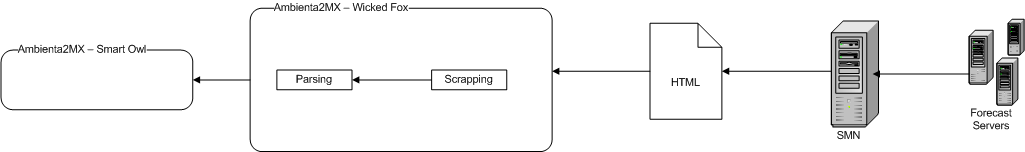
\includegraphics[width=22.5cm,height=12cm]{./images/DiagramaWickedFox.png}
			  \caption{Diagrama General de Wicked Fox}
			\end{figure}
	  	\end{landscape}
	  \newpage
    \paragraph{Éste módulo presenta una gran importancia debido a que actualmente se carece de un servicio a nivel nacional que brinde información meteorológica con cierta veracidad, si bien es cierto que otros sistemas extraen información de datos tomados por centrales mexicanas, el costo de éstos suele ser elevado.}
    \paragraph{La extracción de la información se ejecutará \emph{al vuelo}, es decir, éste proceso se ejecutará cada que se pidan datos con un margen no mayor a una hora de cierta localidad o ubicación del territorio nacional.}
    \paragraph{Para poder hacer uso de éste módulo es necesario brindar la información de la localidad via latitud/longitud o bien, a través de la localidad descrita, éstos datos serán proporcionados y resueltos por el módulo \textbf{\emph{Fast Eagle}} descrito anteriormente.}
      